%%% Copyright (C) 2015-2024 Vincent Goulet
%%%
%%% Ce fichier fait partie du projet
%%% «Rédaction avec LaTeX»
%%% https://gitlab.com/vigou3/formation-latex-ul
%%%
%%% Cette création est mise à disposition sous licence
%%% Attribution-Partage dans les mêmes conditions 4.0
%%% International de Creative Commons.
%%% https://creativecommons.org/licenses/by-sa/4.0/

\documentclass[aspectratio=169,10pt,xcolor=x11names,french]{beamer}
  \usepackage{babel}
  \usepackage[autolanguage]{numprint}
  \usepackage{amsmath}
  \usepackage[mathrm=sym]{unicode-math}  % polices math
  \usepackage{changepage}                % page licence
  \usepackage{tabularx}                  % page licence
  \usepackage{booktabs}                  % beaux tableaux
  \usepackage{fontawesome5}              % icônes
  \usepackage{awesomebox}                % \tipbox et autres
  \usepackage{listings}                  % code source
  \usepackage[export]{adjustbox}         % cadre autour image
  \usepackage[overlay,absolute]{textpos} % couvertures
  \usepackage{metalogo}                  % logo \XeLaTeX

  %% ==========================================
  %%  Informations de publication
  %%  (titre et al. dans couverture-avant.tex)
  %% ==========================================
  \title{Rédaction avec \LaTeX --- Premier pas}
  \author{Vincent Goulet}
  \renewcommand{\year}{2024}
  \renewcommand{\month}{03}
  \newcommand{\ctanurl}{https://ctan.org/pkg/formation-latex-ul}
  \newcommand{\reposurl}{https://gitlab.com/vigou3/formation-latex-ul}

  %% =======================
  %%  Apparence du document
  %% =======================

  %% Thème Beamer
  \usetheme{metropolis}
  \metroset{subsectionpage=progressbar}

  %% Polices de caractères
  \setsansfont{Fira Sans Book}
  [
    BoldFont = {Fira Sans SemiBold},
    ItalicFont = {Fira Sans Book Italic},
    BoldItalicFont = {Fira Sans SemiBold Italic}
  ]
  \setmathfont{Fira Math}
  \newfontfamily\titlefontOS{FiraSans}
  [
    Extension = .otf,
    UprightFont = *-Book,
    BoldFont = *-SemiBold,
    BoldItalicFont = *-SemiBoldItalic,
    Scale = 1.0,
    Numbers = OldStyle
  ]
  \newfontfamily\titlefontFC{FiraSans}
  [
    Extension = .otf,
    UprightFont = *-Book,
    BoldFont = *-SemiBold,
    BoldItalicFont = *-SemiBoldItalic,
    Scale = 1.0,
    Numbers = Uppercase
  ]
  \newfontfamily\lucida{Lucida Bright OT}
  [
    Scale = 0.92
  ]
  \usepackage[babel=true]{microtype}

  %% Police Computer Modern pour exemple de police par défaut
  \newfontfamily\CM{cmunrm}
  [
    Extension = .otf,
    ItalicFont = cmunci,
    BoldFont = cmunrb,
    BoldItalicFont = cmunbi,
    Scale = 1.1
  ]
  \newfontfamily\CMtt{cmuntt}
  [
    Extension = .otf,
    Scale = 1.1
  ]

  %% Police STIX Two pour exemple de police moderne
  \newfontfamily\stixtwo{STIXTwoText}
  [
    Extension = .otf,
    UprightFont = *-Regular,
    Scale = 1,
  ]

  %% Couleurs
  \definecolor{comments}{rgb}{0.5,0.55,0.6} % commentaires
  \definecolor{link}{rgb}{0,0.4,0.6}        % liens internes
  \definecolor{url}{rgb}{0.6,0,0}           % liens externes
  \definecolor{rouge}{rgb}{0.9,0,0.1}       % bandeau rouge UL
  \definecolor{or}{rgb}{1,0.8,0}            % bandeau or UL
  \colorlet{codebg}{LightYellow1}           % fond code R
  \colorlet{prompt}{Orchid4}                % invite de commande
  \colorlet{alert}{mLightBrown} % alias de couleur Metropolis
  \colorlet{dark}{mDarkTeal}    % alias de couleur Metropolis
  \colorlet{code}{mLightGreen}  % alias de couleur Metropolis
  \colorlet{shadecolor}{codebg}

  %% Hyperliens
  \hypersetup{%
    pdfauthor = {Vincent Goulet},
    pdftitle = {Rédaction avec LaTeX - Premiers pas},
    colorlinks = true,
    linktocpage = true,
    urlcolor = {url},
    linkcolor = {link},
    citecolor = {citation},
    pdfpagemode = {UseOutlines},
    pdfstartview = {Fit}}
  \setlength{\XeTeXLinkMargin}{1pt}

  %% Affichage de la table des matières du PDF
  \usepackage{bookmark}
  \bookmarksetup{%
    open = true,
    depth = 3,
    numbered = true}

  %% Paramétrage de babel pour les guillemets
  \frenchbsetup{og=«, fg=»}

  %% Sections de code source
  \lstloadlanguages{[LaTeX]TeX}
  \lstset{language=[LaTeX]TeX,
    basicstyle=\small\ttfamily\NoAutoSpacing,
    keywordstyle=\mdseries,
    commentstyle=\color{comments},
    emphstyle=\color{alert}\bfseries,
    moredelim=[is][\color{prompt}]{---}{-},
    escapeinside=`',
    extendedchars=true,
    showstringspaces=false,
    backgroundcolor=\color{LightYellow1},
    frame=leftline,
    framerule=2pt,
    framesep=5pt,
    xleftmargin=7.4pt
  }

  %%% =========================
  %%%  Nouveaux environnements
  %%% =========================

  %% Environnements pour les demo de code; tirés du document
  %% principal. (L'environnement 'eqxample' ajoute des filets de part
  %% et d'autre du bloc pour illustrer les marges.)
  \newenvironment{demo}{%
    \begin{beamercolorbox}[wd=\linewidth,sep=6pt]{block body example}}
    {\end{beamercolorbox}}
  \newenvironment{texample}[1][0.45\linewidth]{%
    \noindent\begin{minipage}{#1}%
      \def\producing{\end{minipage}\hfill\begin{minipage}{\dimexpr0.9\linewidth-#1}%
        \hbox\bgroup\kern-.2pt%
        \vbox\bgroup\parindent0pt\relax
        % The 3pt is to cancel the -\lineskip from \displ@y
        \abovedisplayskip3pt \abovedisplayshortskip\abovedisplayskip
        \belowdisplayskip0pt \belowdisplayshortskip\belowdisplayskip
        \noindent}
    }{%
      \par
      % Ensure that a lonely \[\] structure doesn't take up width less than
      % \hsize.
      \hrule height0pt width\hsize
      \egroup\kern-.2pt\egroup
    \end{minipage}%
    \par
  }
  \newenvironment{eqxample}{%
    \noindent\begin{minipage}{.45\linewidth}%
      \def\producing{\end{minipage}\hfill\begin{minipage}{.45\linewidth}%
        \hbox\bgroup\kern-.2pt\vrule width.2pt%
        \vbox\bgroup\parindent0pt\relax
        % The 3pt is to cancel the -\lineskip from \displ@y
        \abovedisplayskip3pt \abovedisplayshortskip\abovedisplayskip
        \belowdisplayskip0pt \belowdisplayshortskip\belowdisplayskip
        \noindent}
    }{%
      \par
      % Ensure that a lonely \[\] structure doesn't take up width less than
      % \hsize.
      \hrule height0pt width\hsize
      \egroup\vrule width.2pt\kern-.2pt\egroup
    \end{minipage}%
    \par
  }

  %% Simplfication de l'environnement 'quote' de beamer
  \renewenvironment{quote}{%
    \begin{beamercolorbox}[wd=\linewidth,sep=6pt]{block body example}}
    {\end{beamercolorbox}}

  %% Exercices
  \newenvironment{exercice}{%
    \begin{frame}[fragile=singleslide]
      \frametitle{\faCogs\; Exercice}}{\end{frame}}

  %% =====================
  %%  Nouvelles commandes
  %% =====================

  %% Noms de fonctions, code, environnement, etc.
  \newcommand{\code}[1]{\textcolor{code}{\texttt{#1}}}
  \newcommand{\fichier}[1]{\code{#1}}
  \newcommand{\class}[1]{\textbf{#1}}
  \newcommand{\pkg}[1]{\textbf{#1}}
  \newcommand{\link}[2]{\href{#1}{#2~\raisebox{-0.2ex}{\faExternalLink*}}}

  %% Pour documenter des commandes LaTeX; dérivé de memoir.cls
  \def\bs{\code{\char`\\}}
  \newcommand{\meta}[1]{%
    \ensuremath\langle{\normalfont\itshape #1\/}\ensuremath\rangle}
  \newcommand{\marg}[1]{%
    {\ttfamily\char`\{}\meta{#1}{\ttfamily\char`\}}}
  \newcommand{\oarg}[1]{%
    {\ttfamily\char`\[}\meta{#1}{\ttfamily\char`\]}}
  \newcommand{\cs}[1]{\code{\char`\\#1}}

  %% Identification de la licence CC BY-SA.
  \newcommand{\ccbysa}{\mbox{%
    \faCreativeCommons\kern0.1em%
    \faCreativeCommonsBy\kern0.1em%
    \faCreativeCommonsSa}~\faCopyright[regular]\relax}

  %% Lien vers Gitlab dans la page de notices
  \newcommand{\viewsource}[1]{%
    \href{#1}{\faGitlab\ Voir sur GitLab}}

  %%% =======
  %%%  Varia
  %%% =======

  %% Longueurs pour la composition de la page couverture.
  \newlength{\banderougewidth} \newlength{\banderougeheight}
  \newlength{\bandeorwidth}    \newlength{\bandeorheight}
  \newlength{\imageheight}
  \newlength{\logoheight}

\begin{document}

%%% Copyright (C) 2015-2023 Vincent Goulet
%%%
%%% Ce fichier fait partie du projet
%%% «Rédaction avec LaTeX»
%%% https://gitlab.com/vigou3/formation-latex-ul
%%%
%%% Cette création est mise à disposition sous licence
%%% Attribution-Partage dans les mêmes conditions 4.0
%%% International de Creative Commons.
%%% https://creativecommons.org/licenses/by-sa/4.0/

%% Normes de présentation visuelle 2018
%%
%% - grille de 8 unités de haut
%% - 1 mesure = 1/8 d'unité
%% - bande identitaire de 1 mesure placée au bas de la 7e unité
%% - logo haut de 4 mesures avec blancs de deux mesures en haut et
%%   en bas
%% - blanc équivalent à la largeur du blason à droite du logo
%% - bande or de la largeur du logo + blanc à droite
%%
%% Dimensions du logo UL
%%
%% hauteur: 128
%% largeur totale: 310
%% largeur blason: 100
%% valeur clé: (310 + 100)/128 = 3.2031125
%%
%% Dimensions de l'image
%%
%% hauteur: 55 mesures - 1pt (filet) = 54.9191919 mesures
%% largeur: 160mm
%% ratio largeur/hauteur: 160/77.23

\begingroup
\TPGrid{16}{64}
\textblockorigin{0mm}{0mm}
\setlength{\parindent}{0mm}
\setlength{\imageheight}{54.9191919\TPVertModule}
\setlength{\logoheight}{4\TPVertModule}
\setlength{\bandeorwidth}{3.203125\logoheight}
\setlength{\banderougewidth}{\paperwidth}
\addtolength{\banderougewidth}{-\bandeorwidth}
\setlength{\bandeorheight}{\TPVertModule}
\setlength{\banderougeheight}{\TPVertModule}
\setlength{\textwidth}{\paperwidth}
\addtolength{\textwidth}{-2\TPHorizModule}

\def\titlefmt{%
  \titlefontOS\bfseries\fontsize{24}{24}\selectfont%
  Rédaction avec
  \lucida\mdseries%
  {\textbackslash}title%
  \raisebox{-6pt}{\fontsize{48}{48}\selectfont%
    \{%
    \fontsize{40}{40}\selectfont%
    \LaTeX
    \fontsize{48}{48}\selectfont%
    \}\par}}
\def\subtitlefmt{%
  \titlefontOS\bfseries\fontsize{10}{11}\selectfont%
  Premiers pas\par}
\def\authorfmt{%
  \titlefontOS\bfseries\fontsize{14}{14}\selectfont%
  Vincent Goulet\par}
\def\affiliation{%
  \titlefontOS\mdseries\fontsize{10}{11}\selectfont%
  Professeur titulaire \\
  École d'actuariat, Université Laval}
\def\edition{%
  \titlefontOS\mdseries\fontsize{10}{11}\selectfont%
  Édition {\titlefontFC\year}.\month}

%%%
%%% Page de titre
%%%

\begin{frame}[plain]
  %% bandeau identitaire
  \begin{textblock*}{\paperwidth}[0,1](0mm,56\TPVertModule)
    \textcolor{rouge}{\rule{\banderougewidth}{\banderougeheight}}% % bande rouge
    \textcolor{or}{\rule{\bandeorwidth}{\bandeorheight}}           % bande or
  \end{textblock*}

  %% logo UL
  \begin{textblock*}{\bandeorwidth}(\banderougewidth,58\TPVertModule)
    \includegraphics[height=\logoheight,keepaspectratio=true]{ul_p}
  \end{textblock*}

  %% image de fond
  \begin{textblock*}{\paperwidth}(0mm,0mm)
    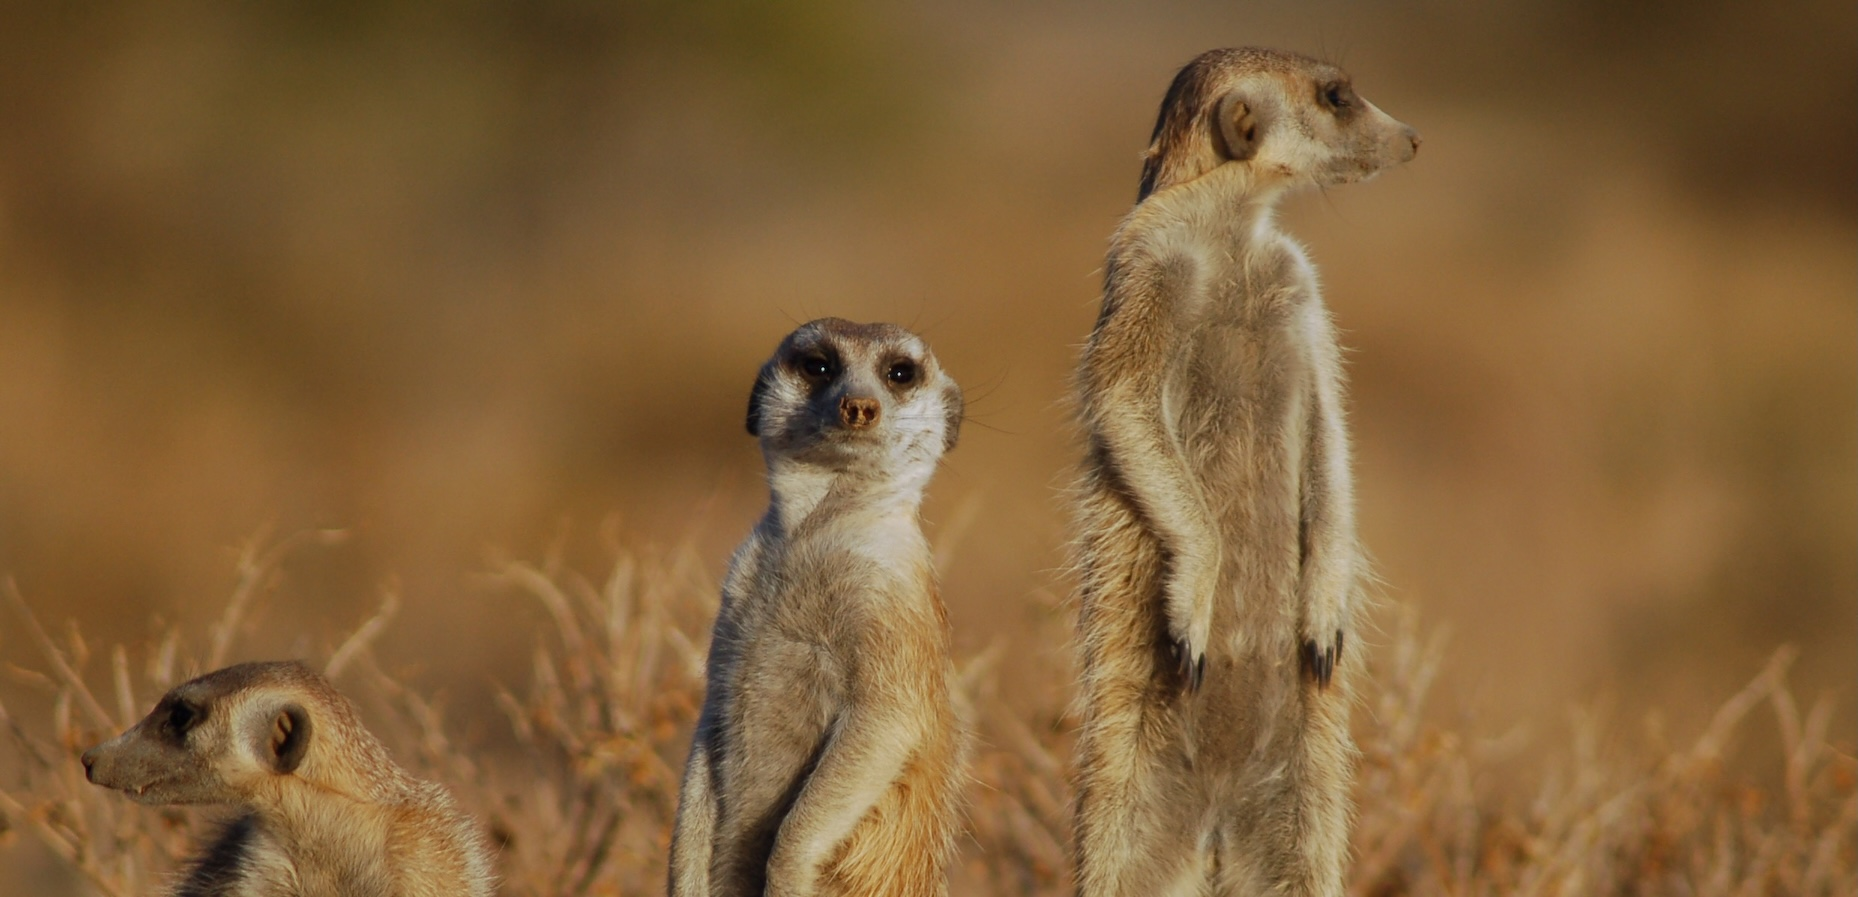
\includegraphics[height=\imageheight,width=\paperwidth]{images/Suricates_Namibia-2-diapos}
  \end{textblock*}

  %% titre
  \begin{textblock*}{\banderougewidth}(0.8\TPHorizModule,4\TPVertModule)
    \textcolor{black!10}{\titlefmt}
  \end{textblock*}

  %% sous-titre (premiers pas)
  \begin{textblock*}{\banderougewidth}(0.8\TPHorizModule,13\TPVertModule)
    \textcolor{black!10}{\subtitlefmt}
  \end{textblock*}
\end{frame}

%%%
%%% Page frontispice
%%%

\begin{frame}[plain]
  %% titre
  \begin{textblock*}{\banderougewidth}(0.8\TPHorizModule,4\TPVertModule)
    \titlefmt
  \end{textblock*}

  %% sous-titre
  \begin{textblock*}{\banderougewidth}(0.8\TPHorizModule,13\TPVertModule)
    \subtitlefmt
  \end{textblock*}

  %% auteur
  \begin{textblock*}{\textwidth}(0.8\TPHorizModule,28\TPVertModule)
    \authorfmt
  \end{textblock*}

  %% affiliation
  \begin{textblock*}{\textwidth}(0.8\TPHorizModule,33\TPVertModule)
    \affiliation
  \end{textblock*}

  %% édition
  \begin{textblock*}{\textwidth}(0.8\TPHorizModule,58\TPVertModule)
    \edition
  \end{textblock*}
\end{frame}
\endgroup

%%% Local Variables:
%%% TeX-master: "formation-latex-ul-diapos"
%%% TeX-engine: xetex
%%% coding: utf-8
%%% End:

%%% Copyright (C) 2015-2024 Vincent Goulet
%%%
%%% Ce fichier fait partie du projet
%%% «Rédaction avec LaTeX»
%%% https://gitlab.com/vigou3/formation-latex-ul
%%%
%%% Cette création est mise à disposition sous licence
%%% Attribution-Partage dans les mêmes conditions 4.0
%%% International de Creative Commons.
%%% https://creativecommons.org/licenses/by-sa/4.0/

\begin{frame}[t,plain,fragile=singleslide]
  \tiny
  \vspace*{10mm}

  \begin{adjustwidth}{15mm}{15mm}
    {\ccbysa} 2015-{\year} par {\insertauthor}. «{\inserttitle}» est
    mis à disposition sous licence
    \href{https://creativecommons.org/licenses/by-sa/4.0/deed.fr}{%
      Attribution-Partage dans les mêmes conditions 4.0 International}
    de Creative Commons. En vertu de cette licence, vous êtes autorisé
    à:
    \begin{itemize}
    \item \textbf{partager} --- copier, distribuer et communiquer le
      matériel par tous moyens et sous tous formats;
    \item \textbf{adapter} --- remixer, transformer et créer à partir du
      matériel pour toute utilisation, y compris commerciale.
    \end{itemize}
    L'Offrant ne peut retirer les autorisations concédées par la licence
    tant que vous appliquez les termes de cette licence.

    Selon les conditions suivantes: \par
    \begin{tabularx}{\linewidth}{@{}l>{\raggedright\arraybackslash}X@{}}
      \raisebox{-11pt}{\fontsize{16}{16}\selectfont\faCreativeCommonsBy}
      & \textbf{Attribution} --- Vous devez créditer l'œuvre, intégrer
        un lien vers la licence et indiquer si des modifications ont été
        effectuées à l'œuvre. Vous devez indiquer ces informations par
        tous les moyens raisonnables, sans toutefois suggérer que
        l'Offrant vous soutient ou soutient la façon dont vous avez utilisé
        son œuvre. \\
      \raisebox{-11pt}{\fontsize{16}{16}\selectfont\faCreativeCommonsSa}
      & \textbf{Partage dans les mêmes conditions} --- Dans le cas où vous
        effectuez un remix, que vous transformez, ou créez à partir du
        matériel composant l'œuvre originale, vous devez diffuser l'œuvre modifiée dans
        les mêmes conditions, c'est-à-dire avec la même licence avec laquelle
        l'œuvre originale a été diffusée.
    \end{tabularx}

    \textbf{Code source} \\
    \viewsource{\reposurl}

    \textbf{Couverture} \\
    Suricates (\emph{Suricata suricatta}) en Namibie. Parfois surnommé
    «sentinelle du désert», ce petit carnivore vit dans le sud-ouest
    de l'Afrique. Très prolifique, le suricate vit en groupes
    familiaux au sein d'une colonie. Crédit photo: {\textcopyright}
    Sara\&Joachim\&Mebe,
    \href{https://creativecommons.org/licenses/by-sa/2.0/deed.fr}{CC
      BY-SA 2.0} via
    \href{https://commons.wikimedia.org/w/index.php?curid=15305478}{%
      Wikimedia Commons}.

    Concept original du titre: Marie-Ève Guérard.
  \end{adjustwidth}
\end{frame}

%%% Local Variables:
%%% TeX-master: "formation-latex-ul-diapos"
%%% TeX-engine: xetex
%%% coding: utf-8
%%% End:

%%% Copyright (C) 2015-2023 Vincent Goulet
%%%
%%% Ce fichier fait partie du projet
%%% «Rédaction avec LaTeX»
%%% https://gitlab.com/vigou3/formation-latex-ul
%%%
%%% Cette création est mise à disposition sous licence
%%% Attribution-Partage dans les mêmes conditions 4.0
%%% International de Creative Commons.
%%% https://creativecommons.org/licenses/by-sa/4.0/

\begin{frame}
  \frametitle{Prérequis à cette formation}

  \begin{adjustwidth}{8mm}{10mm}
    \begin{enumerate}
    \item Installer une distribution {\LaTeX} sur votre poste de
      travail; je recommande la distribution
      \link{https://tug.org/texlive}{{\TeX}~Live}
      \begin{itemize}
      \item \link{https://youtu.be/uJFbhQkDbU8}{%
          Vidéo d'installation sur macOS}
      \item \link{https://youtu.be/wO2FlNmye14}{%
          Vidéo d'installation sur Windows}
      \end{itemize}
    \item Composer un premier document très simple de type \emph{Hello
        World!}
      \begin{itemize}
        \normalsize
      \item \link{https://youtu.be/1XKh0f6hFks}{%
          Démonstration vidéo avec TeXShop sur macOS}
      \item \link{https://youtu.be/EIwsQHJhpOQ}{%
          Démonstration vidéo avec Texmaker sur Windows}
      \end{itemize}
    \end{enumerate}
  \end{adjustwidth}
\end{frame}

%%% Local Variables:
%%% TeX-master: "formation-latex-ul-diapos"
%%% TeX-engine: xetex
%%% coding: utf-8
%%% End:


%%% Copyright (C) 2015-2024 Vincent Goulet
%%%
%%% Ce fichier fait partie du projet
%%% «Rédaction avec LaTeX»
%%% https://gitlab.com/vigou3/formation-latex-ul
%%%
%%% Cette création est mise à disposition sous licence
%%% Attribution-Partage dans les mêmes conditions 4.0
%%% International de Creative Commons.
%%% https://creativecommons.org/licenses/by-sa/4.0/

\section{Présentation de {\TeX} et {\LaTeX}}

\begin{frame}
  \frametitle{Ce que c'est}
  \begin{columns}
    \begin{column}{.5\textwidth}
      \begin{itemize}
      \item {\TeX} est un système de mise en page (\emph{typesetting})
        ou de préparation de documents
      \item {\LaTeX} est un ensemble de macro-commandes pour faciliter
        l'utilisation de {\TeX}
      \item Langage de balisage (\emph{Markup Language}) pour indiquer
        la mise en forme du texte
      \item Accent mis sur la production de documents de grande
        qualité à la typographie soignée (surtout pour les
        mathématiques)
      \end{itemize}
    \end{column}
    \begin{column}{.5\textwidth}
      \centering\vspace*{3ex}
      \includegraphics[width=\linewidth]{images/knuth} \\
      \footnotesize Donald Knuth, créateur de \TeX
    \end{column}
  \end{columns}
\end{frame}

\begin{frame}
  \frametitle{Ce que ce n'est pas}
  \begin{tabular}{lcl}
    Un traitement de texte & \faArrowRight & priorité accordée
                                             à la qualité de
                                             la mise en page \\[6pt]
    WYSIWYG & \faArrowRight & plutôt What You See Is What
                              You \emph{Mean} \\[6pt]
    Incompatible & \faArrowRight & format identique sur tous
                                   les systèmes d'exploitation \\[6pt]
    Instable & \faArrowRight & noyau arrivé à maturité \\[6pt]
    Imprévisible & \faArrowRight & {\LaTeX} fait ce qu'on
                                   lui demande, ni plus, ni moins
  \end{tabular}
\end{frame}

\begin{frame}
  \frametitle{Quelques choses simples à réaliser avec {\LaTeX}}

  \begin{itemize}
  \item Page de titre
  \item Table des matières
  \item Numérotation des pages
  \item Figures et tableaux: disposition, numérotation, renvois
  \item Équations mathématiques: disposition, numérotation, renvois
  \item Citations et composition de la bibliographie
  \item Coupure de mots
  \item Document recto verso
  \end{itemize}
\end{frame}

\begin{frame}[fragile=singleslide]
  \frametitle{Faits amusants}
  \begin{itemize}
  \item {\TeX} est aujourd'hui considéré exempt de bogue
  \item Récompense si vous en trouvez un!
  \item Numéro de version de {\TeX} converge vers $\pi$:
\begin{lstlisting}
---$- tex --version
TeX 3.141592653 (TeX Live 2023)
kpathsea version 6.3.5
Copyright 2023 D.E. Knuth.
[...]
\end{lstlisting} %$
  \end{itemize}
\end{frame}

\begin{frame}
  \frametitle{Processus de création d'un document {\LaTeX}}
  \Huge
  \begin{minipage}[t]{0.25\textwidth}
    \centering
    \faFile*[regular] \\ \bigskip
    \small
    rédaction du texte et balisage avec un \alert{éditeur de texte}
  \end{minipage}
  \hfill\faArrowRight\hfill
  \begin{minipage}[t]{0.25\textwidth}
    \centering
    \faCogs \\  \bigskip
    \small
    compilation avec un \alert{moteur} {\TeX} depuis la ligne de commande
  \end{minipage}
  \hfill\faArrowRight\hfill
  \begin{minipage}[t]{0.3\textwidth}
    \centering
    \faFilePdf[regular] \\  \bigskip
    \small
    visualisation avec une visionneuse PDF (Aperçu,
    SumatraPDF, etc.)
  \end{minipage}
\end{frame}

\begin{exercice}
  Démarrer le logiciel \alert{Texmaker} (Windows), \alert{TeXShop}
  (macOS) ou tout autre éditeur ou logiciel intégré de rédaction de
  votre choix.

  \begin{enumerate}
  \item Ouvrir et compiler le fichier \fichier{exercice-minimal.tex}.
    Comparer le texte du fichier au résultat produit.
  \item Ajouter du texte en français (avec accents), recompiler et
    observer le résultat.
  \end{enumerate}
\end{exercice}

\begin{exercice}
  Question de voir ce que {\LaTeX} peut faire, compiler le document
  élaboré \fichier{exercice-demo.tex} de la manière suivante:
  \begin{enumerate}[i)]
  \item une fois avec \code{LaTeX};
  \item une fois avec \code{BibTeX};
  \item deux à trois fois avec \code{LaTeX}.
  \end{enumerate}
\end{exercice}

%%% Local Variables:
%%% TeX-master: "formation-latex-ul-diapos"
%%% TeX-engine: xetex
%%% coding: utf-8
%%% End:

%%% Copyright (C) 2015-2023 Vincent Goulet
%%%
%%% Ce fichier fait partie du projet
%%% «Rédaction avec LaTeX»
%%% https://gitlab.com/vigou3/formation-latex-ul
%%%
%%% Cette création est mise à disposition sous licence
%%% Attribution-Partage dans les mêmes conditions 4.0
%%% International de Creative Commons.
%%% https://creativecommons.org/licenses/by-sa/4.0/

\section{Principes de base}

\begin{frame}
  \frametitle{Rédaction}

  L'apparence du document est prise en charge par {\LaTeX} et
  il est généralement préférable de ne pas la modifier.

  \begin{itemize}
  \item On se concentre sur le \alert{contenu} et la \alert{structure} du
    document
  \item Mots séparés par une ou plusieurs \alert{espaces}
  \item Paragraphes séparés par une ou plusieurs \alert{lignes blanches}
  \item Utilisation de \alert{commandes} pour indiquer la structure du texte
  \end{itemize}
\end{frame}

\begin{frame}[fragile=singleslide]
  \frametitle{Caractères réservés}

  \begin{itemize}
  \item Caractères réservés par {\TeX}:
    \begin{quote}
      \code{\#~\$~\&~\string~~\_~\string^~\%~\{~\}}
    \end{quote}
  \item Pour les utiliser, précéder par «\bs»
    \begin{demo}
      \begin{texample}
\begin{lstlisting}
L'augmentation de 2~\$
représente une hausse
de 5~\%.
\end{lstlisting}
        \producing
        L'augmentation de 2~\$ représente une
        hausse de 5~\%.
      \end{texample}
    \end{demo}
  \end{itemize}
\end{frame}

\begin{frame}[fragile=singleslide]
  \frametitle{Structure d'un document {\LaTeX}}

  Un fichier source {\LaTeX} est toujours composé de deux parties.

  \begin{minipage}{0.2\linewidth}
    \begin{minipage}{\linewidth}
      \hfill préambule \quad
      \rule[-10mm]{1pt}{21mm}
    \end{minipage} \\[5mm]
    \begin{minipage}{\linewidth}
      \hfill corps \quad
      \rule[-15mm]{1pt}{30mm}
    \end{minipage}
  \end{minipage}
  \hfill
  \begin{minipage}{0.75\linewidth}
\begin{lstlisting}[emph={documentclass,begin,end,document}]
\documentclass[11pt,french]{article}
  \usepackage{babel}
  \usepackage[autolanguage]{numprint}
  \usepackage[utf8]{inputenc}
  \usepackage[T1]{fontenc}

\begin{document}

Lorem ipsum dolor sit amet, consectetur
adipiscing elit. Donec quam nulla, bibendum
vitae ipsum vel, fermentum pellentesque orci.

\end{document}
\end{lstlisting}
  \end{minipage}
\end{frame}

\begin{frame}[fragile=singleslide]
  \frametitle{Commandes}
  \begin{itemize}
  \item Débutent toujours par «\bs»
  \item Exemples de syntaxe
\begin{lstlisting}
\LaTeX                     % aucun argument
\emph{toujours}            % un argument obligatoire
\section*{Introduction}    % effet modifié
\rule[6pt]{5mm}{2pt}       % un argument optionnel, deux obligatoires
\end{lstlisting}
   \item Commande sans argument: le nom se termine par tout
    caractère qui n'est \alert{pas une lettre} (y compris l'espace!)
  \item Portée d'une commande limitée à la zone entre \code{\{~\}}
  \end{itemize}
\end{frame}

\begin{frame}[fragile=singleslide]
  \frametitle{Environnements}
  \begin{itemize}
  \item Délimités par
\begin{lstlisting}
\begin`\marg{environnement}'
   ...
\end`\marg{environnement}'
    \end{lstlisting}
  \item Contenu de l'environnement traité différemment du reste du texte
  \item Changements s'appliquent uniquement à l'intérieur de
    l'environnement
  \end{itemize}
\end{frame}

\begin{frame}[fragile]
  \frametitle{{\LaTeX} en français}

  Il faut charger un certain nombre de paquetages pour franciser \LaTeX.

  \begin{itemize}
  \item \pkg{babel}: traduction des mots-clés prédéfinis,
    typographie française, coupure de mots, document multilingue
  \item \pkg{inputenc} et \pkg{fontenc}: lettres accentuées dans le
    code source (pdf{\LaTeX} seulement)
  \item \pkg{icomma}: virgule comme séparateur décimal
  \item \pkg{numprint}: espace comme séparateur des milliers
  \end{itemize}
\end{frame}

\begin{exercice}
  Modifier le fichier \fichier{exercice-commandes.tex} afin de
  produire le texte ci-dessous.

  \bigskip
  \centering
  \fbox{\includegraphics[viewport=108 551 502 665,%
    clip=true,width=0.9\linewidth]{auxdoc/exercice_commandes-solution}}
\end{exercice}

%%% Local Variables:
%%% TeX-master: "formation-latex-ul-diapos"
%%% TeX-engine: xetex
%%% coding: utf-8
%%% End:

%%% Copyright (C) 2015-2024 Vincent Goulet
%%%
%%% Ce fichier fait partie du projet
%%% «Rédaction avec LaTeX»
%%% https://gitlab.com/vigou3/formation-latex-ul
%%%
%%% Cette création est mise à disposition sous licence
%%% Attribution-Partage dans les mêmes conditions 4.0
%%% International de Creative Commons.
%%% https://creativecommons.org/licenses/by-sa/4.0/

\section{Organisation d'un document}

\begin{frame}[plain]
  \tipbox{Utilisez impérativement les commandes {\LaTeX} pour
    identifier les différentes parties (la structure) d'un document.}
\end{frame}

\begin{frame}[fragile]
  \frametitle{Titre et page de titre}
  {\LaTeX} peut composer une page de titre automatiquement à partir
  des informations pertinentes.

  \begin{lstlisting}
%% préambule
\title{`\meta{Titre du document}'}
\author{`\meta{Prénom Nom}'}
\date{`\meta{date du jour}'}          % automatique si omise

%% corps du document
\maketitle
  \end{lstlisting}
\end{frame}

\begin{frame}[fragile=singleslide]
  \frametitle{Sections}
  \begin{itemize}
  \item Découpage du document en sections
\begin{lstlisting}
\part{`\meta{titre}'}
\chapter{`\meta{titre}'}
\section{`\meta{titre}'}
\subsection{`\meta{titre}'}
\end{lstlisting}
  \item Numérotation automatique
    \begin{demo}
      \begin{minipage}{0.45\linewidth}
\begin{lstlisting}
\section{Hypothèses}
\end{lstlisting}
      \end{minipage}
      \hfill
      \begin{minipage}{0.45\linewidth}
        \includegraphics[height=0.8\baselineskip,keepaspectratio]{images/section-num}
      \end{minipage}
    \end{demo}
  \item Sans la numérotation
    \begin{demo}
      \begin{minipage}{0.45\linewidth}
\begin{lstlisting}
\section*{Hypothèses}
\end{lstlisting}
      \end{minipage}
      \hfill
      \begin{minipage}{0.45\linewidth}
        \includegraphics[height=0.8\baselineskip,keepaspectratio]{images/section-non-num}
      \end{minipage}
    \end{demo}
  \end{itemize}
\end{frame}

\begin{frame}[fragile=singleslide]
  \frametitle{Annexes}

  Les annexes sont des sections ou des chapitres avec une numérotation
  alphanumérique (A, A.1, ...)
  \begin{itemize}
  \item \cs{appendix} identifie les sections suivantes comme des annexes
  \item Dans le titre, «Chapitre» changé pour «Annexe» le cas échéant
  \end{itemize}
\end{frame}

\begin{frame}[fragile=singleslide]
  \frametitle{Table des matières}

  La commande \cs{tableofcontents} produit automatiquement la table
  des matières.

  \begin{itemize}
  \item Requiert plusieurs compilations
  \item Sections non numérotées pas incluses
  \item Avec \pkg{hyperref}, produit également la table des
    matières du fichier PDF
  \end{itemize}
\end{frame}

\begin{frame}
  \frametitle{Étiquettes et renvois automatiques}

  Ne \alert{jamais} renvoyer manuellement à un numéro de section,
  d'équation, de tableau, etc.

  \begin{itemize}
  \item Étiquetter un élément avec \cs{label}
  \item Faire référence par son étiquette avec \cs{ref}
  \item Requiert 2 à 3 compilations
  \end{itemize}
\end{frame}

\begin{frame}[fragile=singleslide]
  \frametitle{Exemple (code source)}

  \begin{lstlisting}[emph={\label,\ref}]
\section{Définitions}
\label{sec:definitions}

Lorem ipsum dolor sit amet, consectetur
adipiscing elit. Duis in auctor dui. Vestibulum
ut, placerat ac, adipiscing vitae, felis.

\section{Historique}

Tel que vu à la section \ref{sec:definitions},
on a...
\end{lstlisting}
\end{frame}

\begin{frame}
  \frametitle{Exemple (résultat)}

  \fbox{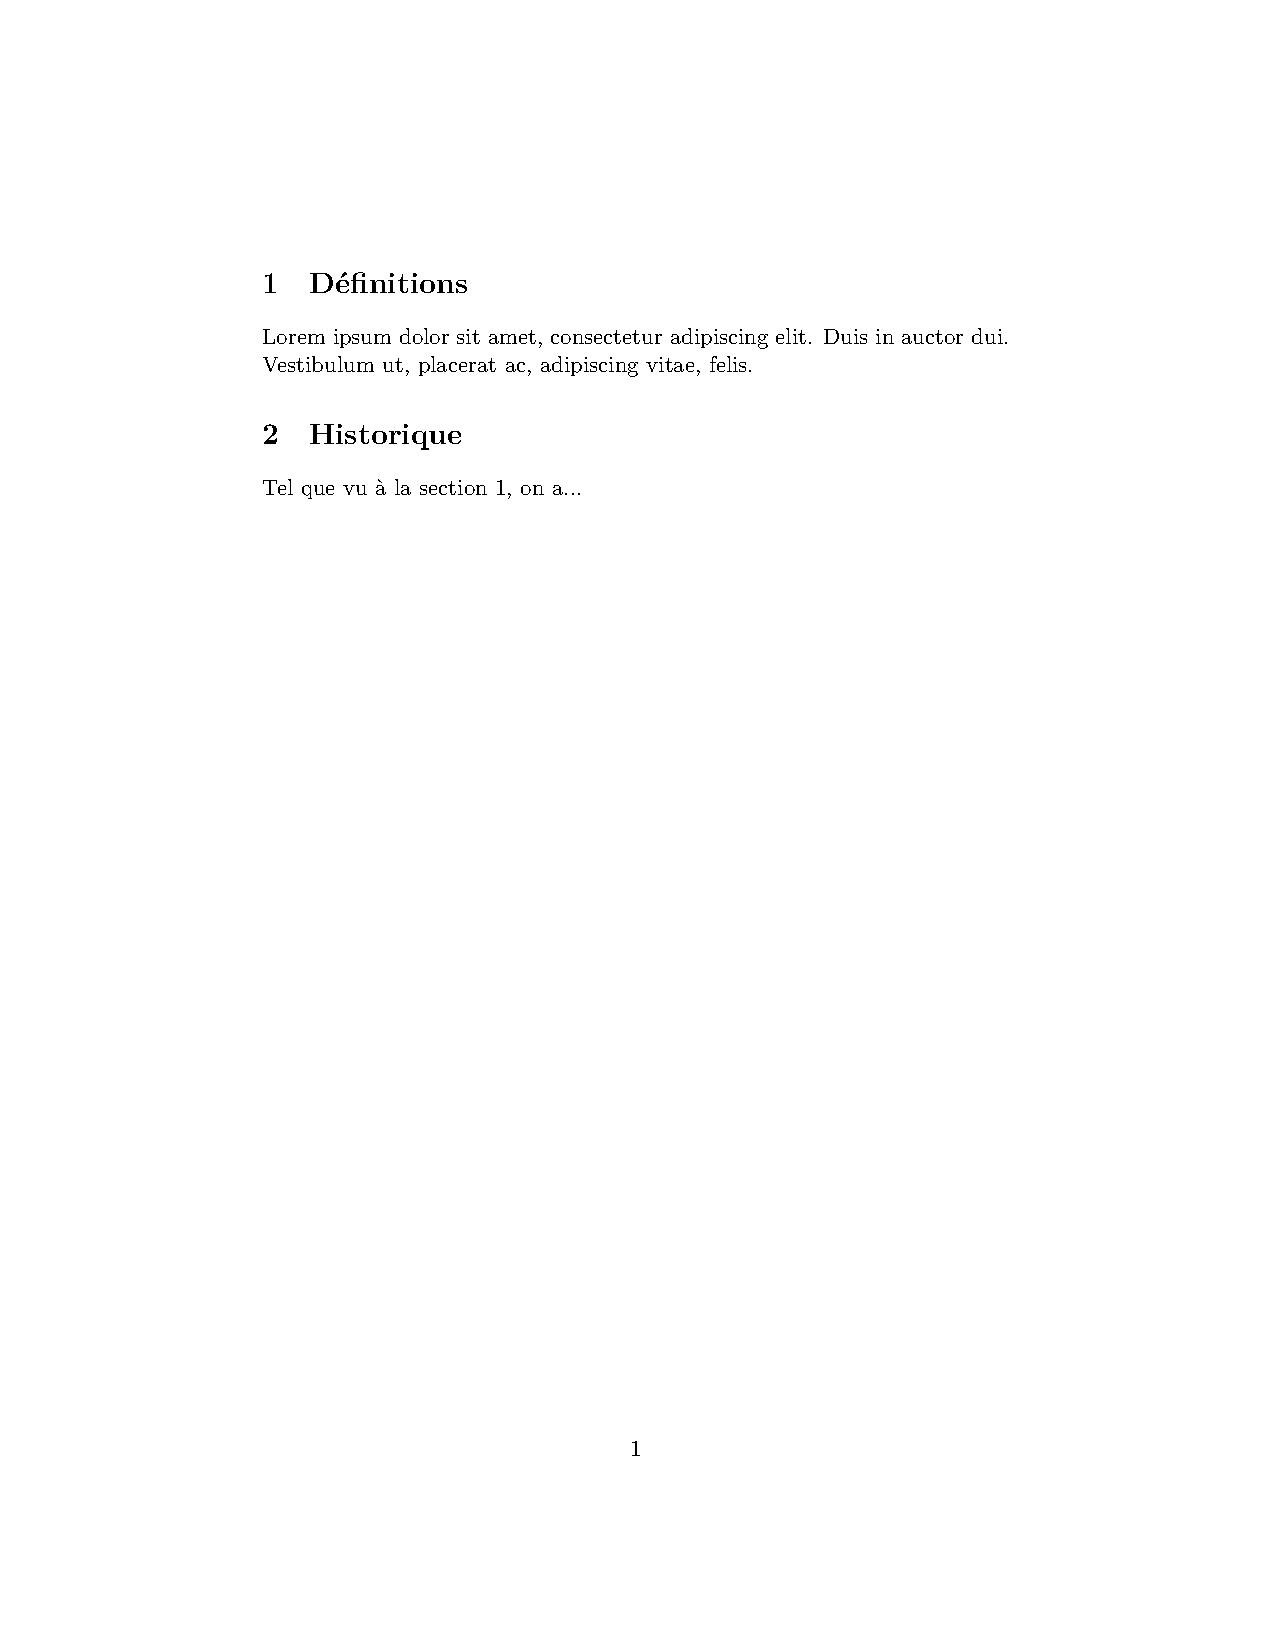
\includegraphics[viewport=124 550 484 664,clip=true,width=0.98\linewidth]{auxdoc/exemple-renvoi}}
\end{frame}

\begin{exercice}
  Utiliser le fichier \fichier{exercice-renvois.tex}.
  \begin{enumerate}
  \item Insérer dans le texte un renvoi au numéro d'une section.
  \item Activer le paquetage \pkg{hyperref} avec l'option
    \code{colorlinks} et comparer l'effet d'utiliser \cs{ref} ou
    \cs{autoref} pour le renvoi.
  \end{enumerate}
\end{exercice}

%%% Local Variables:
%%% TeX-master: "formation-latex-ul-diapos"
%%% TeX-engine: xetex
%%% coding: utf-8
%%% End:

%%% Copyright (C) 2015-2024 Vincent Goulet
%%%
%%% Ce fichier fait partie du projet
%%% «Rédaction avec LaTeX»
%%% https://gitlab.com/vigou3/formation-latex-ul
%%%
%%% Cette création est mise à disposition sous licence
%%% Attribution-Partage dans les mêmes conditions 4.0
%%% International de Creative Commons.
%%% https://creativecommons.org/licenses/by-sa/4.0/

\section{Apparence et disposition du texte}

\begin{frame}
  \frametitle{Police de caractères}

  Par défaut, {\LaTeX} compose les documents dans la police
  {\CM Computer Modern}.

  \begin{itemize}
  \item Dans un premier temps, n'essayez pas de changer la police de
    caractère du document
  \item Commandes pour modifier les \alert{attributs} de la police
    (famille, forme, graisse)
    \medskip

    par ex.:
    {
      \small
      \begin{tabular}[t]{l}
        \cs{rmfamily} \\ \CM romain
      \end{tabular} \quad
      \begin{tabular}[t]{l}
        \cs{ttfamily} \\ \CMtt largeur fixe
      \end{tabular} \quad
      \begin{tabular}[t]{l}
        \cs{itshape} \\ \CM\itshape italique
      \end{tabular} \quad
      \begin{tabular}[t]{l}
        \cs{bfseries} \\ \CM\bfseries gras
      \end{tabular}
    }
  \item Commandes pour modifier la \alert{taille} du texte
    \medskip

    par ex.:
    {
      \small
      \begin{tabular}[t]{l}
        \cs{footnotesize} \\ \CM\footnotesize très petit
      \end{tabular} \quad
      \begin{tabular}[t]{l}
        \cs{small} \\ \CM\small petit
      \end{tabular} \quad
      \begin{tabular}[t]{l}
        \cs{large} \\ \CM\large grand
      \end{tabular} \quad
      \begin{tabular}[t]{l}
        \cs{Large} \\ \CM\Large très grand
      \end{tabular}
    }
  \end{itemize}
\end{frame}

\begin{frame}[fragile=singleslide]
  \frametitle{Italique}
  \begin{itemize}
  \item Une des propriétés les plus utilisées dans le texte
  \item Commande sémantique:
\begin{lstlisting}
\emph`\marg{texte}'
\end{lstlisting}
  \item Pas de commande pour souligner en {\LaTeX\dots} et ce n'est
    pas une omission!
  \end{itemize}
\end{frame}

\begin{frame}[fragile]
  \frametitle{Listes}
  \begin{itemize}
  \item Deux principales sortes de listes:
    \begin{enumerate}
    \item \alert{à puce} avec environnement \code{itemize}
    \item \alert{numérotée} avec environnement \code{enumerate}
    \end{enumerate}
  \item Possible de les imbriquer les unes dans les autres
  \item Marqueurs adaptés automatiquement jusqu'à 4 niveaux
  \pause

\begin{lstlisting}
\begin{itemize}
\item Deux principales sortes de listes:
  \begin{enumerate}
  \item à puce avec environnement \texttt{itemize}
  \item numérotée avec environnement \texttt{enumerate}
  \end{enumerate}
\item Possible de les imbriquer les unes dans les autres
\item Marqueurs adaptés automatiquement jusqu'à 4 niveaux
\end{itemize}
\end{lstlisting}
  \end{itemize}
\end{frame}

\begin{frame}[fragile]
  \frametitle{Notes de bas de page}
  \begin{itemize}
  \item Note de bas de page insérée avec la commande
\begin{lstlisting}
\footnote`\marg{texte de la note}'
\end{lstlisting}
  \item Commande doit suivre immédiatement le texte à annoter
  \item Numérotation et disposition automatiques
  \end{itemize}
\end{frame}

\begin{frame}[fragile=singleslide]
  \frametitle{Code source}
  \begin{itemize}
  \item Environnement \code{verbatim}
\begin{lstlisting}
\begin{verbatim}
Texte disposé exactement tel qu'il est saisi
dans une police à largeur fixe
\end{verbatim}
\end{lstlisting}
  \item Pour usage plus intensif, utiliser les paquetages
    \pkg{fancyvrb} ou \pkg{listings}
  \end{itemize}
\end{frame}

\begin{frame}[plain]
  \tipbox{Il est aujourd'hui beaucoup plus facile d'utiliser d'autres
    polices de caractères pour vos documents, surtout avec {\XeLaTeX}.


    Attention, toutefois: peu de polices sont adaptées pour les
    mathématiques.

    Excellents choix modernes: %
    \link{https://ctan.org/pkg/stix2-otf/}{\stixtwo STIX~Two}, %
    \link{https://ctan.org/pkg/fira}{Fira Sans}.}
\end{frame}

\begin{exercice}
  Utiliser le fichier \fichier{exercice-complet.tex}.

  \begin{enumerate}
  \item Étudier le code source du fichier, puis le compiler.
  \item Supprimer l'option \code{article} au chargement de la classe
    et compiler de nouveau le document. Observer l'effet de cette
    option.
  \item Effectuer les modifications suivantes au document.
    \begin{enumerate}[a)]
    \item Dernier paragraphe de la première section, placer toute la
      phrase débutant par \code{«De simple dérivé»} à l'intérieur
      d'une commande \cs{emph}.
    \item Changer la puce des listes pour le symbole \code{\$>\$} en
      activant la commande \cs{frenchbsetup\{ItemLabeli=\$>\$\}} dans
      le préambule.
    \end{enumerate}
  \end{enumerate}
\end{exercice}

%%% Local Variables:
%%% TeX-master: "formation-latex-ul-diapos"
%%% TeX-engine: xetex
%%% coding: utf-8
%%% End:

%%% Copyright (C) 2015-2023 Vincent Goulet
%%%
%%% Ce fichier fait partie du projet
%%% «Rédaction avec LaTeX»
%%% https://gitlab.com/vigou3/formation-latex-ul
%%%
%%% Cette création est mise à disposition sous licence
%%% Attribution-Partage dans les mêmes conditions 4.0
%%% International de Creative Commons.
%%% https://creativecommons.org/licenses/by-sa/4.0/

\section{Tableaux}

\begin{frame}
  \frametitle{De la conception de beaux tableaux}

  Lequel de ces deux tableaux est le plus facile à consulter?
  \begin{center}
  \hfill
  \begin{tabular}{|>{$}c<{$}|>{$}r<{$}|>{$}r<{$}|}
    \hline\hline
    i &
    \multicolumn{1}{c|}{$v$} &
    \multicolumn{1}{c|}{$b_i$} \\
    \hline
    0 & \nombre{91492} &  60 \\
    \hline
    1 &  \nombre{1524} &  60 \\
    \hline
    2 &            25  &  24 \\
    \hline
    3 &             1  & 365 \\
    \hline\hline
  \end{tabular}
  \hfill
  \begin{tabular}{>{$}c<{$}>{$}r<{$}>{$}r<{$}}
    \toprule
    i &
    \multicolumn{1}{c}{$v$} &
    \multicolumn{1}{c}{$b_i$} \\
    \midrule
    0 & \nombre{91492} &  60 \\
    1 &  \nombre{1524} &  60 \\
    2 &            25  &  24 \\
    3 &             1  & 365 \\
    \bottomrule
  \end{tabular}
  \hspace*{\fill}
  \end{center}

  \pause
  Deux règles d'or:
  \begin{enumerate}
  \item \alert{jamais} de filets verticaux
  \item pas de filets doubles
  \end{enumerate}
\end{frame}

\begin{frame}[fragile=singleslide]
  \frametitle{Paquetage essentiel}

  \begin{itemize}
  \item Vous voulez utiliser le paquetage \pkg{booktabs}
\begin{lstlisting}
\usepackage{booktabs}
\end{lstlisting}
  \item Fonctionnalités intégrées dans la classe \class{memoir}
  \end{itemize}
\end{frame}

\begin{frame}[fragile=singleslide]
  \frametitle{Exemple de tableau}

  \begin{center}
    \begin{tabular}{lcrr}
      \toprule
      Produit & Quantité & Prix unitaire (\$) & Prix (\$) \\
      \midrule
      Vis à bois    & 2 & 9,90 & 19,80 \\
      Clous vrillés & 5 & 4,35 & 21,75 \\
      \midrule
      TOTAL         & 7 &      & 41,55 \\
      \bottomrule
    \end{tabular}
  \end{center}

\begin{lstlisting}
\begin{tabular}{lcrr}
  \toprule
  Produit & Quantité & Prix unitaire (\$) & Prix (\$) \\
  \midrule
  Vis à bois    & 2 & 9,90 & 19,80 \\
  Clous vrillés & 5 & 4,35 & 21,75 \\
  \midrule
  TOTAL         & 7 &      & 41,55 \\
  \bottomrule
\end{tabular}
\end{lstlisting}
\end{frame}

%%% Local Variables:
%%% TeX-master: "formation-latex-ul-diapos"
%%% TeX-engine: xetex
%%% coding: utf-8
%%% End:

%%% Copyright (C) 2015-2024 Vincent Goulet
%%%
%%% Ce fichier fait partie du projet
%%% «Rédaction avec LaTeX»
%%% https://gitlab.com/vigou3/formation-latex-ul
%%%
%%% Cette création est mise à disposition sous licence
%%% Attribution-Partage dans les mêmes conditions 4.0
%%% International de Creative Commons.
%%% https://creativecommons.org/licenses/by-sa/4.0/

\section{B.a.-ba des mathématiques}

\begin{frame}[fragile=singleslide]
  \frametitle{Principes de base}
  \begin{itemize}
  \item Décrire des équations mathématiques requiert un «langage» spécial
    \begin{itemize}
    \item il faut informer {\LaTeX} que l'on passe à ce langage
    \item par le biais de modes mathématiques
    \end{itemize}
  \item Important d'utiliser un mode mathématique
    \begin{itemize}
    \item règles de typographie spéciales
    \item espaces gérées automatiquement
    \end{itemize}
  \item Vous voulez utiliser le paquetage \pkg{amsmath}
\begin{lstlisting}
\usepackage{amsmath}
\end{lstlisting}
  \end{itemize}
\end{frame}

\begin{frame}[fragile]
  \frametitle{Modes mathématiques}
  \begin{enumerate}[<+->]
  \item «En ligne» directement dans le texte comme $(a + b)^2 = a^2 +
    2ab + b^2$ en plaçant l'équation entre \verb=$ $=
\begin{lstlisting}
«En ligne» directement dans le texte
comme $(a + b)^2 = a^2 + 2ab + b^2$
\end{lstlisting}
  \item «Hors paragraphe» séparé du texte principal comme
    \begin{equation*}
      \int_0^\infty f(x)\, dx = \sum_{i = 1}^n \alpha_i e^{x_i} f(x_i)
    \end{equation*}
    en utilisant divers types d'environnements
\begin{lstlisting}
«Hors paragraphe» séparé du texte principal comme
\begin{equation*}
  \int_0^\infty f(x)\, dx =
  \sum_{i = 1}^n \alpha_i e^{x_i} f(x_i)
\end{equation*}
\end{lstlisting}
  \end{enumerate}
\end{frame}

\begin{frame}[plain]
  \tipbox{En ligne ou hors paragraphe, les équations font partie intégrante de
    la phrase.

    Les règles de ponctuation usuelles s'appliquent donc aux
    équations. \newline

    \fbox{\includegraphics[width=0.95\linewidth]{images/ponctuation}}}
\end{frame}

\begin{frame}[fragile]
  \frametitle{Quelques règles de base}
  \begin{itemize}
  \item En mode mathématique, {\TeX} écrit automatiquement les
    constantes en romain et les variables en italique
    \begin{demo}
      \begin{texample}
\begin{lstlisting}
$z = 2a + 3y$
\end{lstlisting}
        \producing
        $z = 2a + 3y$
      \end{texample}
    \end{demo}
  \item Espacement entre les éléments géré automatiquement, peu importe
    le code source
    \begin{demo}
      \begin{texample}
\begin{lstlisting}
$z=2 a+3 y$
\end{lstlisting}
        \producing
        $z=2 a+3 y$
      \end{texample}
    \end{demo}
  \end{itemize}
\end{frame}

\begin{frame}[fragile]
  \frametitle{Quelques règles de base (suite)}
  \begin{itemize}
  \item \alert{Ne pas} utiliser le mode mathématique pour obtenir du
    texte en italique!
    \begin{demo}
      \begin{minipage}{0.45\linewidth}
\begin{lstlisting}
\emph{xyz}
\end{lstlisting}
      \end{minipage}
      \hfill
      \begin{minipage}{0.45\linewidth}
        \includegraphics[height=0.8\baselineskip,keepaspectratio]{images/xyz-emph}
      \end{minipage}\par
      \begin{minipage}{0.45\linewidth}
\begin{lstlisting}
$xyz$
\end{lstlisting}
      \end{minipage}
      \hfill
      \begin{minipage}{0.45\linewidth}
        \includegraphics[height=0.8\baselineskip,keepaspectratio]{images/xyz-math}
      \end{minipage}
    \end{demo}
  \item Commande \cs{text} de \pkg{amsmath} pour texte à
    l'intérieur du mode mathématique
    \begin{demo}
      \begin{texample}
\begin{lstlisting}
$x = 0 \text{ si } y < 2$
\end{lstlisting}
        \producing
        $x = 0 \text{ si } y < 2$
      \end{texample}
    \end{demo}
  \end{itemize}
\end{frame}

\begin{frame}[fragile]
  \frametitle{Avant-gout}

  Pouvez-vous interpréter ce code?
\begin{lstlisting}
\begin{equation*}
  \Gamma(\alpha) =
  \sum_{j = 0}^\infty \int_j^{j + 1}
    x^{\alpha - 1} e^{-x}\, dx
\end{equation*}
\end{lstlisting}
  \vspace{18pt}
  \pause

  Fort probablement!
  \begin{equation*}
    \Gamma(\alpha) =
    \sum_{j = 0}^\infty \int_j^{j + 1} x^{\alpha - 1} e^{-x}\, dx
  \end{equation*}
\end{frame}

\begin{exercice}
  Utiliser le fichier \fichier{exercice-mathematiques.tex}.

  \begin{enumerate}
  \item Étudier le code source du fichier, puis le compiler.
  \item Charger le paquetage \pkg{amsfonts} dans le préambule, puis
    remplacer \verb=$R^+$= par \verb=$\mathbb{R}^+$= à la ligne
    débutant par «Le domaine».
  \item À l'aide de la fonction Rechercher et remplacer de l'éditeur
    de texte, remplacer toutes les occurrences du symbole $\theta$ par
    $\lambda$.
  \end{enumerate}
\end{exercice}


%%% Local Variables:
%%% TeX-master: "formation-latex-ul-diapos"
%%% TeX-engine: xetex
%%% coding: utf-8
%%% End:

%%% Copyright (C) 2015-2024 Vincent Goulet
%%%
%%% Ce fichier fait partie du projet
%%% «Rédaction avec LaTeX»
%%% https://gitlab.com/vigou3/formation-latex-ul
%%%
%%% Cette création est mise à disposition sous licence
%%% Attribution-Partage dans les mêmes conditions 4.0
%%% International de Creative Commons.
%%% https://creativecommons.org/licenses/by-sa/4.0/

\section{Et la suite?}

\begin{frame}
  \frametitle{Pour en savoir plus}

  \begin{columns}
    \begin{column}{.6\textwidth}
      Le document de référence fournit des détails additionnels et
      couvre des concepts plus avancés:
      \begin{itemize}
        \small
      \item boites, tableaux et figures
      \item équations mathématiques élaborées
      \item bibliographie et citations
      \item commandes et environnement sur mesure
      \item changement de police
      \item diapositives
      \item etc.
      \end{itemize}
    \end{column}
    \begin{column}{.4\textwidth}
      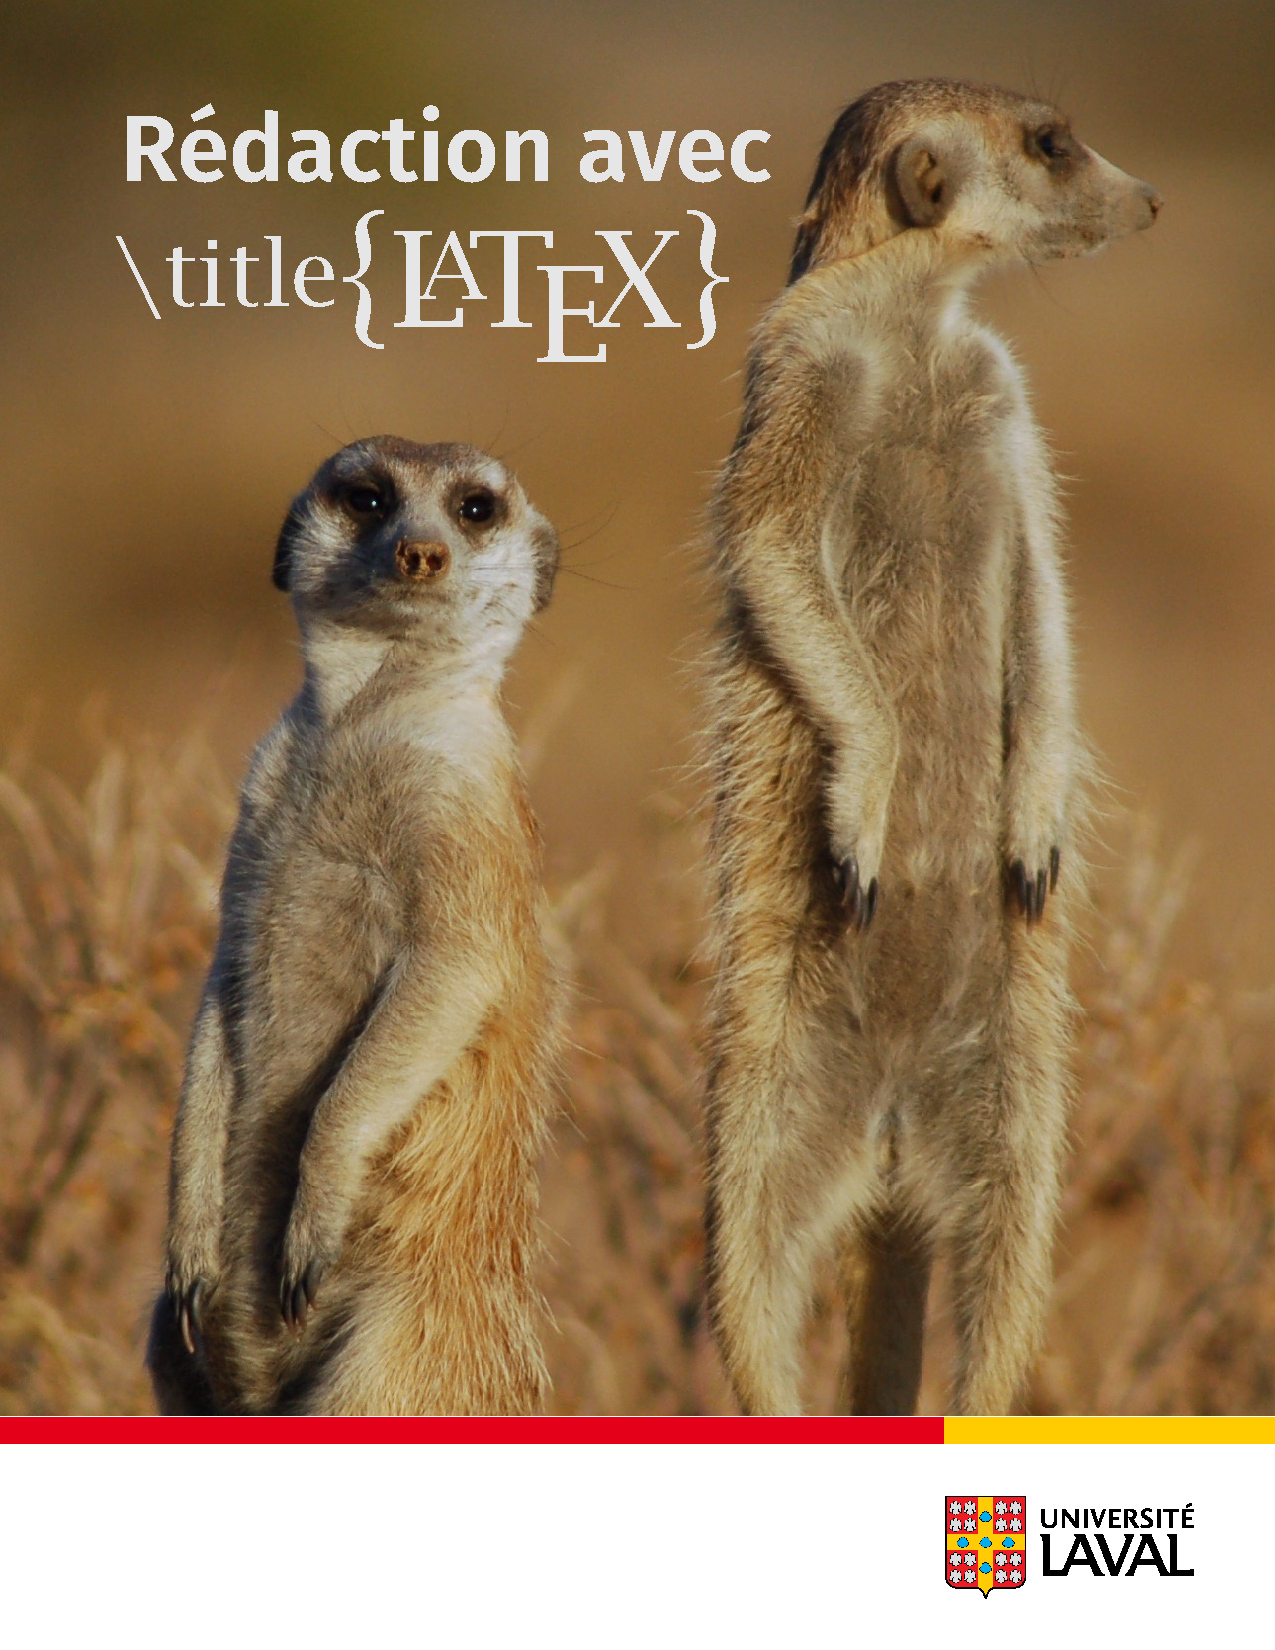
\includegraphics[height=0.8\textheight,frame]{images/formation-latex-ul}
    \end{column}
  \end{columns}
\end{frame}

%%% Local Variables:
%%% TeX-master: "formation-latex-ul-diapos"
%%% TeX-engine: xetex
%%% coding: utf-8
%%% End:


%%% Copyright (C) 2015-2023 Vincent Goulet
%%%
%%% Ce fichier fait partie du projet
%%% «Rédaction avec LaTeX»
%%% https://gitlab.com/vigou3/formation-latex-ul
%%%
%%% Cette création est mise à disposition sous licence
%%% Attribution-Partage dans les mêmes conditions 4.0
%%% International de Creative Commons.
%%% https://creativecommons.org/licenses/by-sa/4.0/

\begin{frame}[plain]
  \begin{adjustwidth}{20mm}{20mm}
    \scriptsize \raggedright %
    Ce document a été produit par le système de mise en page
    {\XeLaTeX} avec la classe \textbf{beamer} et le thème Metropolis.
    Les titres et le texte sont composés en Fira~Sans, les
    mathématiques en Fira~Math et le code informatique en Fira~Mono.
    Les icônes proviennent de la police Font~Awesome.
  \end{adjustwidth}
\end{frame}

%%% Local Variables:
%%% TeX-master: "formation-latex-ul-diapos"
%%% TeX-engine: xetex
%%% coding: utf-8
%%% End:


\end{document}

%%% Local Variables:
%%% TeX-master: t
%%% TeX-engine: xetex
%%% coding: utf-8
%%% End:
